\section{Introduction}
\textcolor{note}{this section is too long}

\label{Section: introduction}
With the increasing demand for continuous video analytics in public safety and transportation, more and more cameras are being deployed to various locations. The video analytics are based on classical computer vision techniques as well as deep convolutional neural networks. In recent years, we have also witnessed the emergence of a large number of excellent models for target detection \cite{trade-offs}, such as FasterRCNN \cite{ren2015faster_rcnn}, RFCN \cite{dai2016r_fcn}, Multibox \cite{szegedy2014multibox}, SSD \cite{liu2016ssd} and YOLO \cite{redmon2016yolo}.

%For the collected video, the classical computer vision and deep neural network technology are generally used for video analytics. 

A video analytics application consists of a \emph{pipeline} of several video processing modules, typically including a decoder, a selective sampling frame application, and a target detector. Such a pipeline always has multiple \emph{knobs}, such as frame rate, resolution, and model (e.g., SSD+\{MobileNet \cite{MobileNetV2}, ResNet \cite{he2016resnet}\}, FasterRCNN+\{ResNet,InceptionResNet \cite{szegedy2016inception}\}). A combination of the knob values is a video analytics \emph{configuration}. The configuration space grows \emph{exponentially} with the number of knobs and their values \cite{jiang2018chameleon}. Since video analytics applications demand intensive computation resources and high accuracy, we pay much attention to the consumption of resources in the calculation process and the accuracy of inference. Therefore, the problem that follows is how to balance \emph{resource consumption} and \emph{accuracy}. Different configurations directly affect accuracy and resource consumption. Using a fixed static high configuration can be very precise, but it can also be a huge drain on resource consumption. Similarly, specifying a low configuration will result in a significant reduction in accuracy.

%Apparently, choosing different configurations will affect resource consumption and accuracy. When at a fixed frame rate, using a complex model with high resolution can obviously and accurately detect the target object, but it also requires more computing resources. Similarly, when using the same model with the same resolution, choosing a lower resolution can reduce the computing resources, and the subsequent cost is the decline of accuracy. Obviously, when the target car (object) is large, a smaller model and a lower resolution can meet the accuracy with a large reduction of resource consumption, while the target car (object) is small, a more complex model and higher resolution are needed to achieve a satisfactory accuracy. And in the case of a highway video analytics, due to the rate of car travel cannot be predicted in advance, so when the car drives slowly (or static) because of the traffic jam, we can choose a lower frame rate (such as 1 FPS) instead of having to use a constant high frame rate throughout whole video. This can significantly reduce resource consumption, but does not affect the accuracy of the video analytics. 


\begin{figure*}[!t]
	\centerline{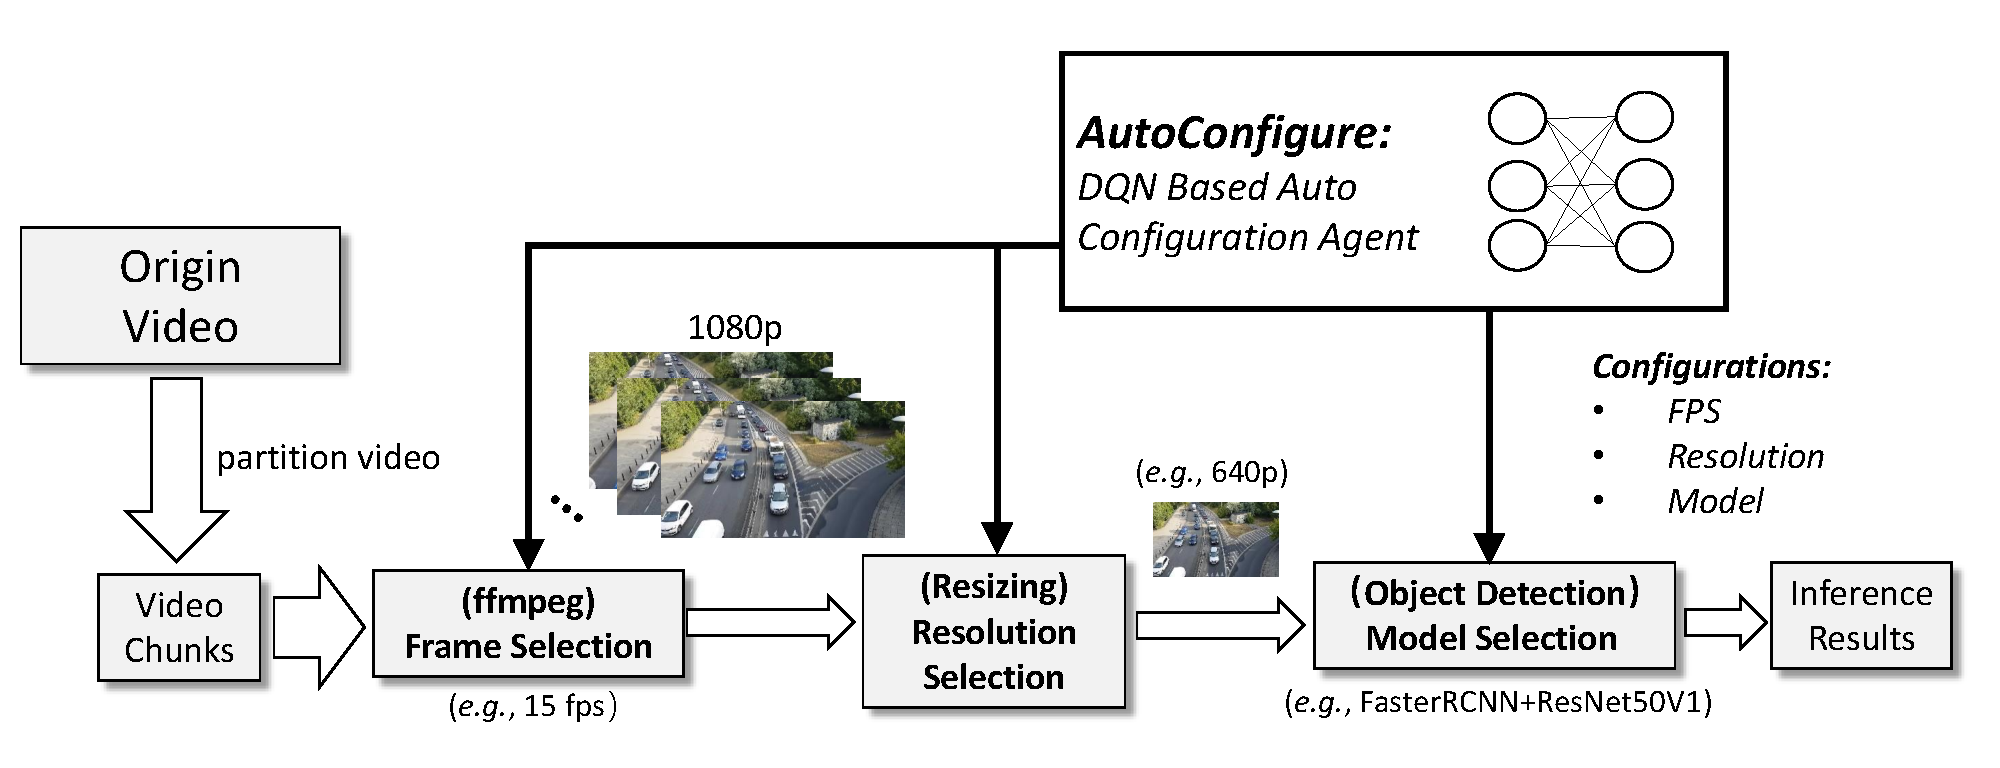
\includegraphics[width=0.9\linewidth]{figures/framework.pdf}}
	%	\vspace{0.2cm}
	\caption{Framework of AutoConfigure architecture}
	\label{fig: framework}
\end{figure*}

%We use~\autoref{fig2} to support that, the data in this figure come from a real road. It can be found that with the decrease of frame rate, the resource consumption can be significantly reduced, but the decrease of accuracy is partly acceptable.

%As shown in~\autoref{fig1}, at a fixed frame rate, using a complex model with high resolution (such as FasterRCNN+InceptionResnet 1024p) can obviously and accurately detect the target object, but it also requires more computing resources. However, when using the same model, choosing a lower resolution can reduce the computing resources, and the subsequent cost is the decline of accuracy. Another example is that choosing a simple model with low resolution (such as FasterRCNN+ResNet50 640p) can significantly reduce resource consumption, although it reduces the accuracy to some extent.

%\begin{figure}[h]
%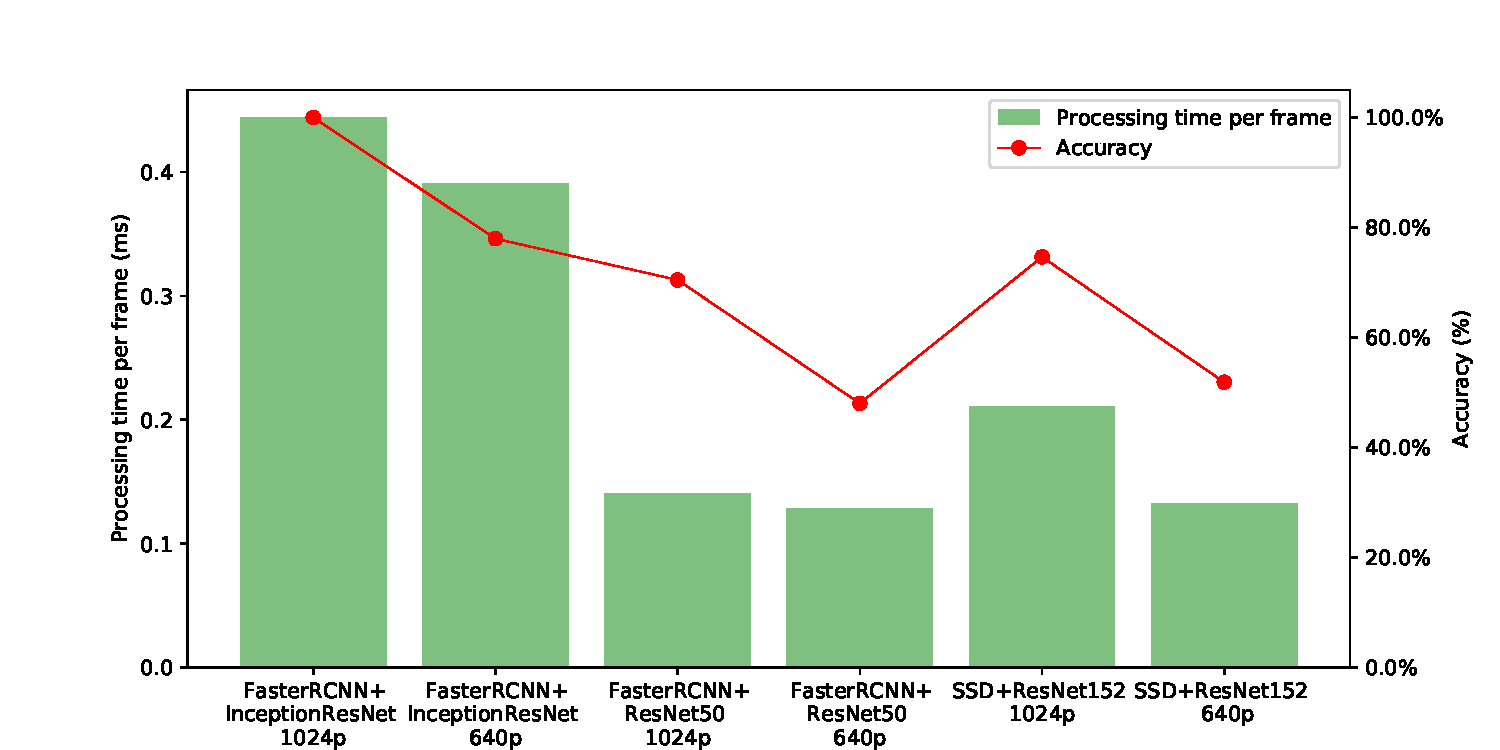
\includegraphics[width=9cm,height=5cm]{figures/figure1.pdf}
%\centering
%\caption{The effect of different models and resolutions on accuracy and processing time at a fixed frame rate.}
%\label{fig1}
%\end{figure}
%
%\begin{figure}[h]
%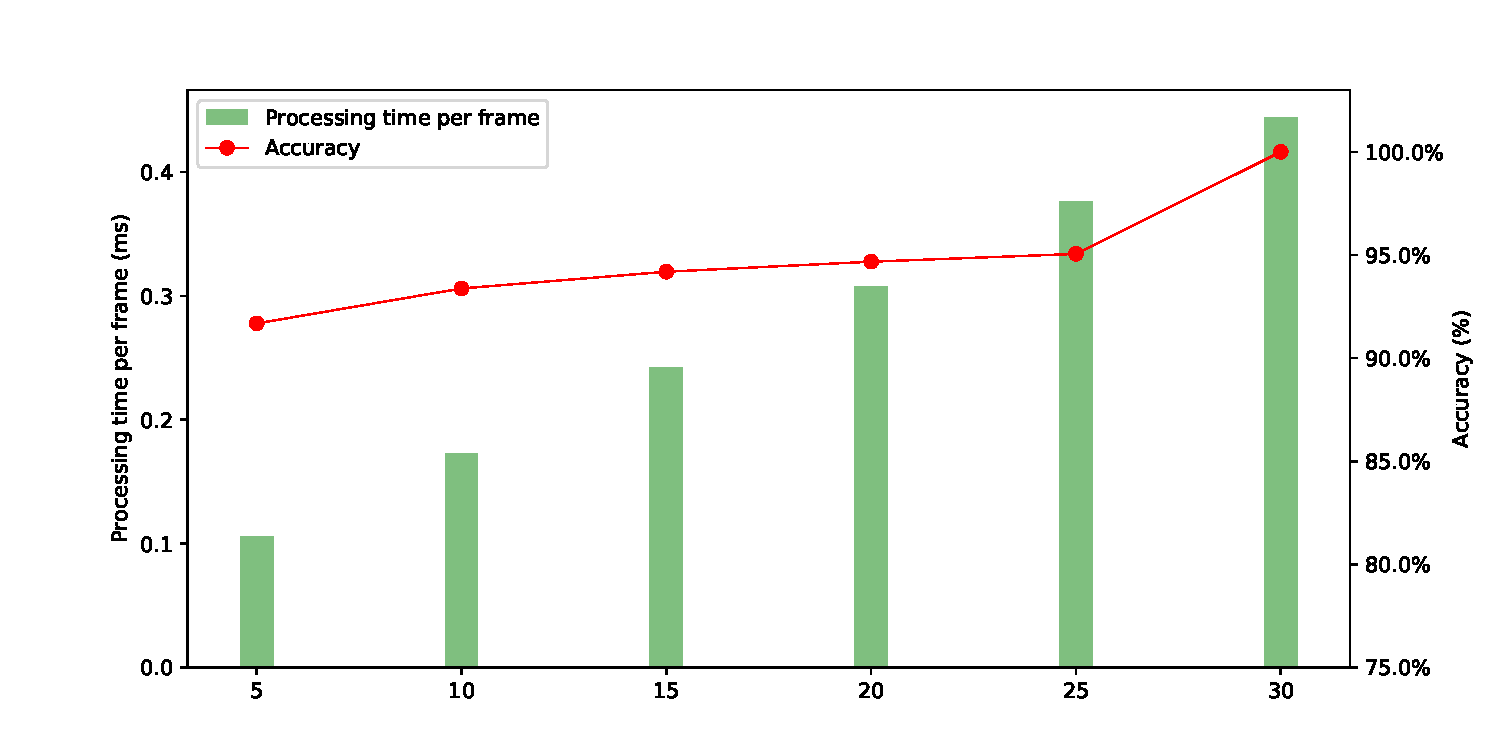
\includegraphics[width=9cm,height=5cm]{figures/figure2.pdf}
%\centering
%\caption{Under the best model, the accuracy and processing time vary with the different frame rate.}
%\label{fig2}
%\end{figure}

The \emph{best} configuration for a video analytics services also varies over time, often at a timescale of minutes or even seconds \cite{jiang2018chameleon}. Hence, our goal is to find a range of ``most appropriate'' configurations that takes up the minimum amount of computing resources and is accurate to the desired threshold. On the one hand, if one only profiles the processing pipeline to choose the best configuration \emph{once}, the application would either waste resources (by picking an expensive configuration) or sacrifice accuracy (by picking a cheap configuration). On the other hand, if one periodically profiles the processing pipeline to find an optimal resource-accuracy \emph{tradeoff} by exhaustive all configurations, it would be prohibitively expensive since the configuration space is extremely large, and thousands of configurations can be combined with just a few knobs.

%The most intuitive way to solve this problem is to find the best solution by exhaustive all configurations, but the number of possible configurations grows exponentially, and thousands of configurations can be combined with just a few knobs, so exhaustive configuration is a highly unrealistic approach.

For a video analytics application, choosing the ``most appropriate'' configuration is a complicated decision-making problem, which is challenging to be solved by rules. An automatic approach is needed, one that is able to learn from video contexts, to decide what is the best configuration for the current video context. The reinforcement learning method is an excellent way to solve this unsupervised complex-environmental problem. In our solution, we tackle the following design challenges.


%Also, one is not provided the well-labeled data on which configuration should be used in which time of the video, meaning this is an unsupervised learning task.

\begin{itemize}	
\item \emph{The best configuration for a video analytics services changes over time with the environment.} The real-world environment is non-stationary; for instance, tracking vehicles when traffic moves quickly requires a much higher frame rate than when traffic moves slowly, but when each condition occurs may vary by hour, minute, or second. As a dynamic video analytics configuration solution, we target to provide a solution that dynamically picks a configuration according to intrusive dynamics of video contexts, i.e., it can \emph{generate} video analytics configuration for video analytics in a different time.

\item \emph{How to significantly reduce the resource cost of periodic configuration profiling.} The cost of periodically profiling often exceeds any resource savings gained by adapting the best configurations we end up selecting. We leverage a Reinforcement Learning-based agent to automatically pick the best configuration periodically, dramatically reducing the profiling cost. 

\item \emph{Lack of well-labeled training data.} In our problem, one is not provided the well-labeled data on which configuration should be used in which time of the video, as in conventional supervised deep learning tasks. In practice, such a video analytics configuration is usually utilized in an online manner, and the solution has to learn from the video contexts automatically. 
\end{itemize}

To address the above challenges, we present a context-driven automatic configuration framework based on reinforcement learning, called AutoConfigure, which can dynamically select the ``most appropriate'' configuration according to intrusive dynamics of video contexts, thus solving this difficult optimal configuration decision problem in a very low-cost way. A brief framework of AutoConfigure is shown in Figure~\ref{fig: framework}. \textcolor{note}{some description?} The main contributions of this paper are summarized as follows.

\begin{itemize}	
\item We design an interactive training environment that can be applied to different video analytics applications. We propose an Deep Q-learning Network-based \cite{DQN} agent to pick the best configuration for video analytics. Also, we define the elements of the RL-based approach, such as actions, states and rewards, to adapt the configuration to current video context.

\item We build a reinforcement learning-based framework to train the agent in the above environment. The agent can learn to choose a ``most appropriate'' configuration for each timestamp of video analytics after iteratively interacting with the environment by feeding the carefully designed reward that considers both accuracy and resources.
 
\item AutoConfigure can achieve 20-30\% higher accuracy with the
same amount of resources, or achieve the same accuracy
with only 50-70\% of the resources. Furthermore, AutoConfigure proves to be more efficient than existing baselines by creating an overhead of less than xx\%\textcolor{note}{(To be tested)} to the overall video analytics services.
\end{itemize}

%The rest of this paper is organized as follows. We discuss related works in Section \ref{Section: related_works}. We present our framework and detailed design in Section \ref{Section: design}. We present our solution's performance in Section \ref{Section: evaluation} and conclude the paper in Section \ref{Section: conclusion}.